%!TEX root = sf_workshop.tex
%

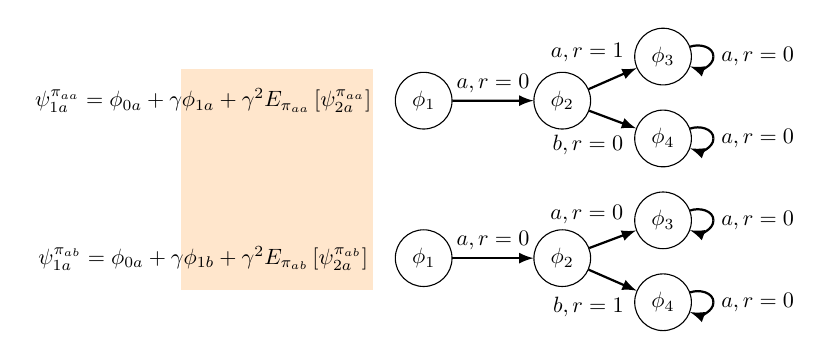
\begin{tikzpicture}[domain=-3:3,scale=0.8, every node/.style={transform shape}]

%\draw (-3.35,2) -- (-.3,2) -- (-.3,-2) -- (-3.35,-2) -- cycle;
%\draw[fill=blue,opacity=0.1] (-3.35,2) rectangle (-.3,-2);
\fill [orange,opacity=.2] (-2.85,2) rectangle (.2,-1.5);

\node[circle,draw=black,minimum size=.9cm](phi1) at (1,    1.5) {$\pmb{\phi}_1$};
\node[circle,draw=black,minimum size=.9cm](phi2) at (3.2, 1.5) {$\pmb{\phi}_2$};
\node[circle,draw=black,minimum size=.9cm](phi3) at (4.8, 2.2) {$\pmb{\phi}_3$};
\node[circle,draw=black,minimum size=.9cm](phi4) at (4.8,.9) {$\pmb{\phi}_4$};

\draw[thick,-latex] (phi1) -- (phi2) node[pos=.5, above] {$a,r=0$};
\draw[thick,-latex] (phi2) -- (phi3) node[pos=.9, above left] {$a,r=1$};
\draw[thick,-latex] (phi2) -- (phi4) node[pos=.9, below left] {$b,r=0$};

\node[anchor=west](phi3out) at (5.6, 2.2) {$a, r=0$};
\path[] (phi3) edge[thick,out=20,in=90] (5.6,2.2)
	   (5.6,2.2) edge[-latex,thick,out=-90,in=-20] (phi3);
	   
\node[anchor=west](phi4out) at (5.6, .9) {$a, r=0$};
\path[] (phi4) edge[thick,out=20,in=90] (5.6,.9)
	   (5.6,.9) edge[-latex,thick,out=-90,in=-20] (phi4);

\node[](sf) at (-2.5,    1.5) {$\pmb{\psi}_{1a}^{\pi_{aa}} = \pmb{\phi}_{0a} + \gamma \pmb{\phi}_{1a} + \gamma^2 \mathbb{E}_{\pi_{aa}} \left[ \pmb{\psi}_{2a}^{\pi_{aa}} \right]$};



\node[circle,draw=black,minimum size=.9cm](phi1) at (1,    -1.) {$\pmb{\phi}_1$};
\node[circle,draw=black,minimum size=.9cm](phi2) at (3.2, -1.) {$\pmb{\phi}_2$};
\node[circle,draw=black,minimum size=.9cm](phi3) at (4.8, -.4) {$\pmb{\phi}_3$};
\node[circle,draw=black,minimum size=.9cm](phi4) at (4.8,-1.7) {$\pmb{\phi}_4$};

\draw[thick,-latex] (phi1) -- (phi2) node[pos=.5, above] {$a,r=0$};
\draw[thick,-latex] (phi2) -- (phi3) node[pos=.9, above left] {$a,r=0$};
\draw[thick,-latex] (phi2) -- (phi4) node[pos=.9, below left] {$b,r=1$};

\node[anchor=west](phi3out) at (5.6, -.4) {$a, r=0$};
\path[] (phi3) edge[thick,out=20,in=90] (5.6,-.4)
	   (5.6,-.4) edge[-latex,thick,out=-90,in=-20] (phi3);
	   
\node[anchor=west](phi4out) at (5.6, -1.7) {$a, r=0$};
\path[] (phi4) edge[thick,out=20,in=90] (5.6,-1.7)
	   (5.6,-1.7) edge[-latex,thick,out=-90,in=-20] (phi4);

\node[](sf) at (-2.5,    -1.) {$\pmb{\psi}_{1a}^{\pi_{ab}} = \pmb{\phi}_{0a} + \gamma \pmb{\phi}_{1b} + \gamma^2 \mathbb{E}_{\pi_{ab}} \left[ \pmb{\psi}_{2a}^{\pi_{ab}} \right]$};

\end{tikzpicture} 
